\documentclass[a4paper, 12pt]{article}

\usepackage{geometry}
\geometry{left=2cm, right=2cm, top=2cm, bottom=2cm}

\usepackage{cmap}
\usepackage{mathtext} 
\usepackage[T2A]{fontenc}
\usepackage[utf8]{inputenc}
\usepackage[english,russian]{babel}	

\usepackage{amsfonts,amssymb,amsthm,mathtools}
\usepackage{amsmath}
\usepackage{icomma} 

\usepackage{graphicx} 
\graphicspath{{picturies/}}
\usepackage{wrapfig}

\usepackage{array,tabularx,tabulary,booktabs}
\usepackage{longtable}
\usepackage{multirow}

\usepackage{caption}
\captionsetup{labelsep=period}

\renewcommand{\phi}{\varphi}
\newcommand{\eps}{\varepsilon}
\newcommand{\parag}[1]{\paragraph*{#1:}}

\newcounter{Points}
\setcounter{Points}{1}
\newcommand{\point}{\arabic{Points}. \addtocounter{Points}{1}}

\author{Радькин Кирилл, Б01-005}
\date{12.02.22}
\title{Лабораторная работа 4.2.3. Интерферометр Релея.}

\begin{document}
\maketitle

\parag {Цель работы} ознакомление с устройством и принципом действия интерферометра Релея и с его применением для измерения показателей преломления газов.

\parag {В работе используются} технический интерферометр ИТР-1, светофильтр, баллон с углекислым газом, сильфон, манометр, краны.

\parag {Экспериментальная установка} ~

\begin{figure}[!h]
    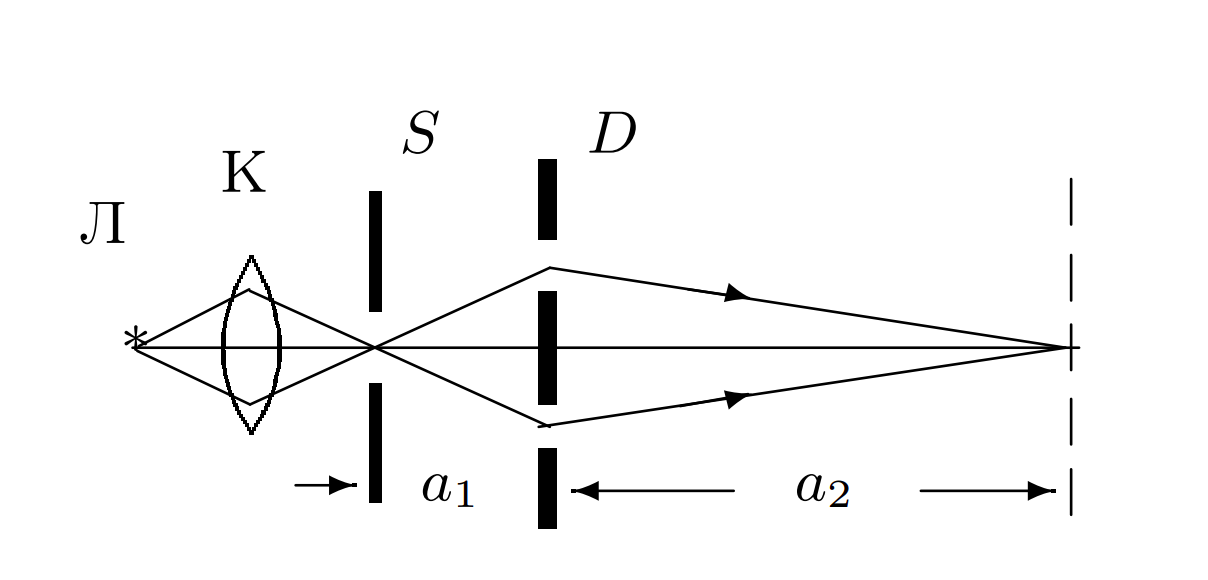
\includegraphics[scale = 0.2]{Workplace.png}
    \centering
    \caption{Принципиальная схема установки для наблюдения дифракции}
    \label{workplace}
\end{figure}

\begin{figure}[!h]
    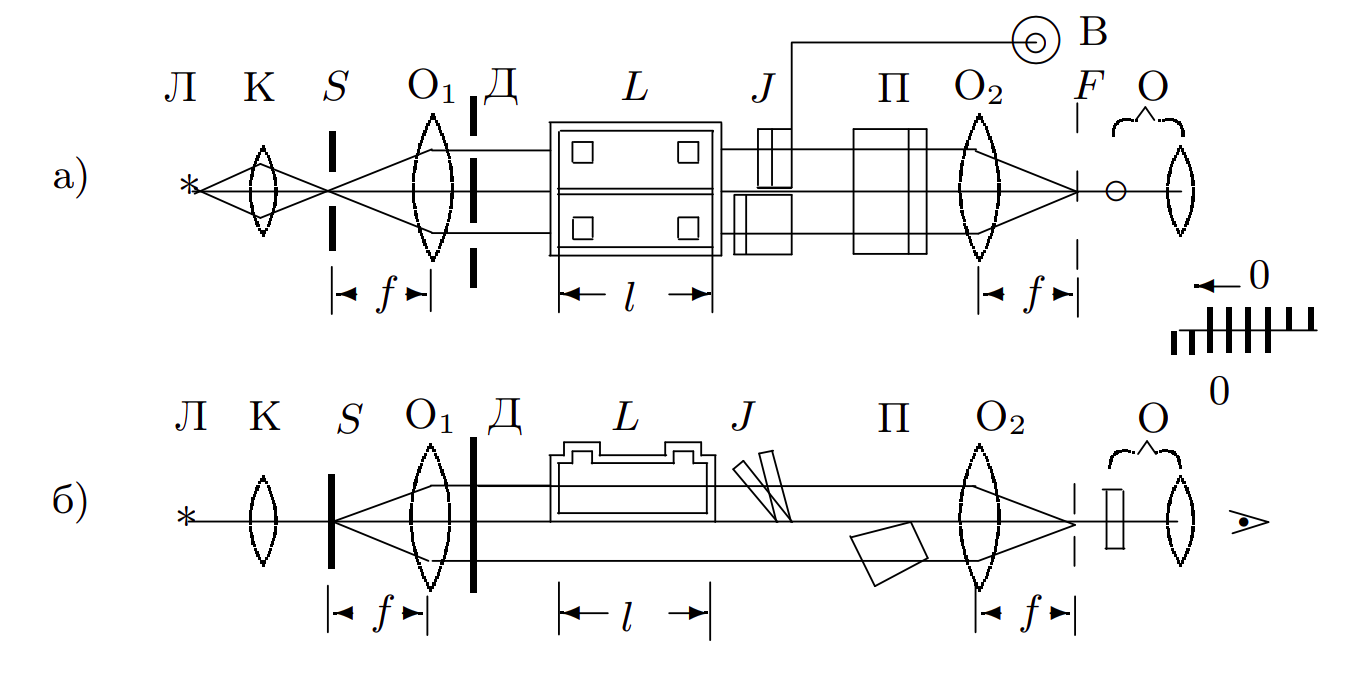
\includegraphics[scale = 0.2]{device.png}
    \centering
    \caption{Устройство интерферометра Релея. а) вид сверху; б) вид сбоку}
    \label{device}
\end{figure}

Интерферометр Релея~---~прибор для измерения разности показателей преломления~---~основан на явлении дифракции света на двух параллельных щелях. Схема прибора представлена на рис. 4 в вертикальной и горизонтальной проекциях. Лампа накаливания Л с помощью конденсора К ярко освещает узкую входную щель S, расположенную в фокусе объектива $O_1$. Коллиматор, состоящий из щели S и объектива $O_1$, посылает параллельный пучок на диафрагму D с двумя вертикальными щелями. Свет, дифрагируя на двойной щели, проходит кювету L, состоящую из двух одинаковых стеклянных камер, в которые вводятся исследуемые газы (в нашей установке — $CO_2$ или воздух). Кювета занимает только верхнюю часть пространства между объективами $O_1$ и $O_2$.

\parag {Ход работы} ~

\begin{enumerate}
    \item Включим осветитель интерферометра в сеть и убедимся, что в поле зрения окуляра видны две системы интерференционных полос.
    \item Уравняем давление в обеих камерах кюветы: первую соединим с атмосферой, открыв краны $К1$ и К2, а вторую (с открытым концом) продуем с помощью груши Г, чтобы
    удалить из неё остатки углекислого газа.
    \item Уравняв давление в камерах, подождем 2–3 минуты, пока выровняются температуры.Установим начало отсчёта, совместив с помощью компенсатора обе системы полос.
    \item Прокалибруем компенсатор в единицах $\lambda$, выделив узкий интервал длин волн с помощью светофильтра. Для этого наденем на оправу окуляра красный светофильт и, последовательно совмещая первую, вторую и т.~д. подвижные полосы с нулевой неподвижной, запишем соответствующие отсчёты по вертикальной шкале и барабану компенсатора.
    
    \begin{tabular}{|c|c|c|c|c|c|c|c|} \hline
        \multicolumn{8}{|c|}{$z, $ мм.} \\ \hline
        0.80 & 1.40 & 1.72 & 2.05 & 2.41 & 2.73 & 3.03 & 3.37 \\ \hline
        3.69 & 4.03 & 4.36 & 4.66 & 4.98 & 5.30 & 5.64 & 5.94 \\ \hline
    \end{tabular}

    \item Запишем длину кюветы $l = 10$ см, длина волны $\lambda = 6700 \buildrel _\circ \over {\mathrm{A}}$, полоса пропускания светофильтра $6200$~---~$7200 \buildrel _\circ \over {\mathrm{A}}$.
    \item Убедимся, что давление воздуха в обеих камерах кюветы атмосферное. Установим сильфон в среднее положение и отсоедините первую камеру от атмосферы, перекрыв кран K1.
    \item Изменяя давление с помощью сильфона и совмещая нулевые полосы, снимем зависимость показаний компенсатора $z$ от перепада давлений $\Delta P$.
    
    \begin{tabular}{|c|c|c|c|c|c|c|c|c|c|c|c|} \hline
        $\Delta P$, мм. в. ст & 1000 & 900 & 800 & 700 & 600 & 500 & 400 & 300 & 200 & 100 & 0 \\ \hline
        $z$, мм. & 4.07 & 3.92 & 3.74 & 3.65 & 3.54 & 3.45 & 3.23 & 3.14 & 3.00 & 2.86 & 2.76 \\ \hline
        $\Delta P$, мм. в. ст & -100 & -200 & -300 & -400 & -500 & -600 & -700 & -800 & -900 & \multicolumn{2}{|c|}{-1000} \\ \hline
        $z$, мм. & 2.55 & 2.46 & 2.36 & 2.19 & 1.99 & 1.86 & 1.72 & 1.53 & 1.29 & \multicolumn{2}{|c|}{1.03} \\ \hline
    \end{tabular}

    \item Соединим первую камеру кюветы с атмосферой, открыв кран K1, и отключим манометр, закрыв кран K2. Заполним углекислым газом камеру с открытым
    концом. Для этого 3–4 раза плавно, чтобы избежать резкого изменения температуры газа при расширении, переведем кран K0 из положения 1 в положение 2.
    \item Снимем зависимость равновесного положения компенсатора от времени, раз в минуту совмещая нулевые полосы, и оценим время установления равновесия.
    
    \begin{tabular}{|c|c|c|c|c|c|c|c|c|c|c|c|} \hline
        $t$, мин. & 0 & 1 & 2 & 3 & 4 & 5 & 6 & 7 & 8 & 9 & 10 \\ \hline
        $z$, мм. & 9.90 & 8.86 & 7.89 & 7.50 & 6.58 & 6.00 & 5.42 & 5.07 & 4.81 & 4.45 & 4.30 \\ \hline
    \end{tabular}

    Повторим измерения, стараясь заполнять кювету как можно более плавно.

    \begin{tabular}{|c|c|c|c|c|c|c|} \hline
        $t$, мин. & 0 & 1 & 2 & 3 & 4 & 5 \\ \hline
        $z$, мм. & 9.99 & 8.73 & 7.78 & 7.37 & 6.82 & 6.25 \\ \hline
    \end{tabular}

    \item Определим температуру $T = 22.2$ $C^{\circ}$ и давление $P = 100.2$ кПа по показаниям лабораторного термометра и барометра.
    \item Построим калибровочный график в координатах $x = m$ (номер совмещённой полосы), $y = z$ (отсчёт по компенсатору).
    
    \begin{figure}[!h]
        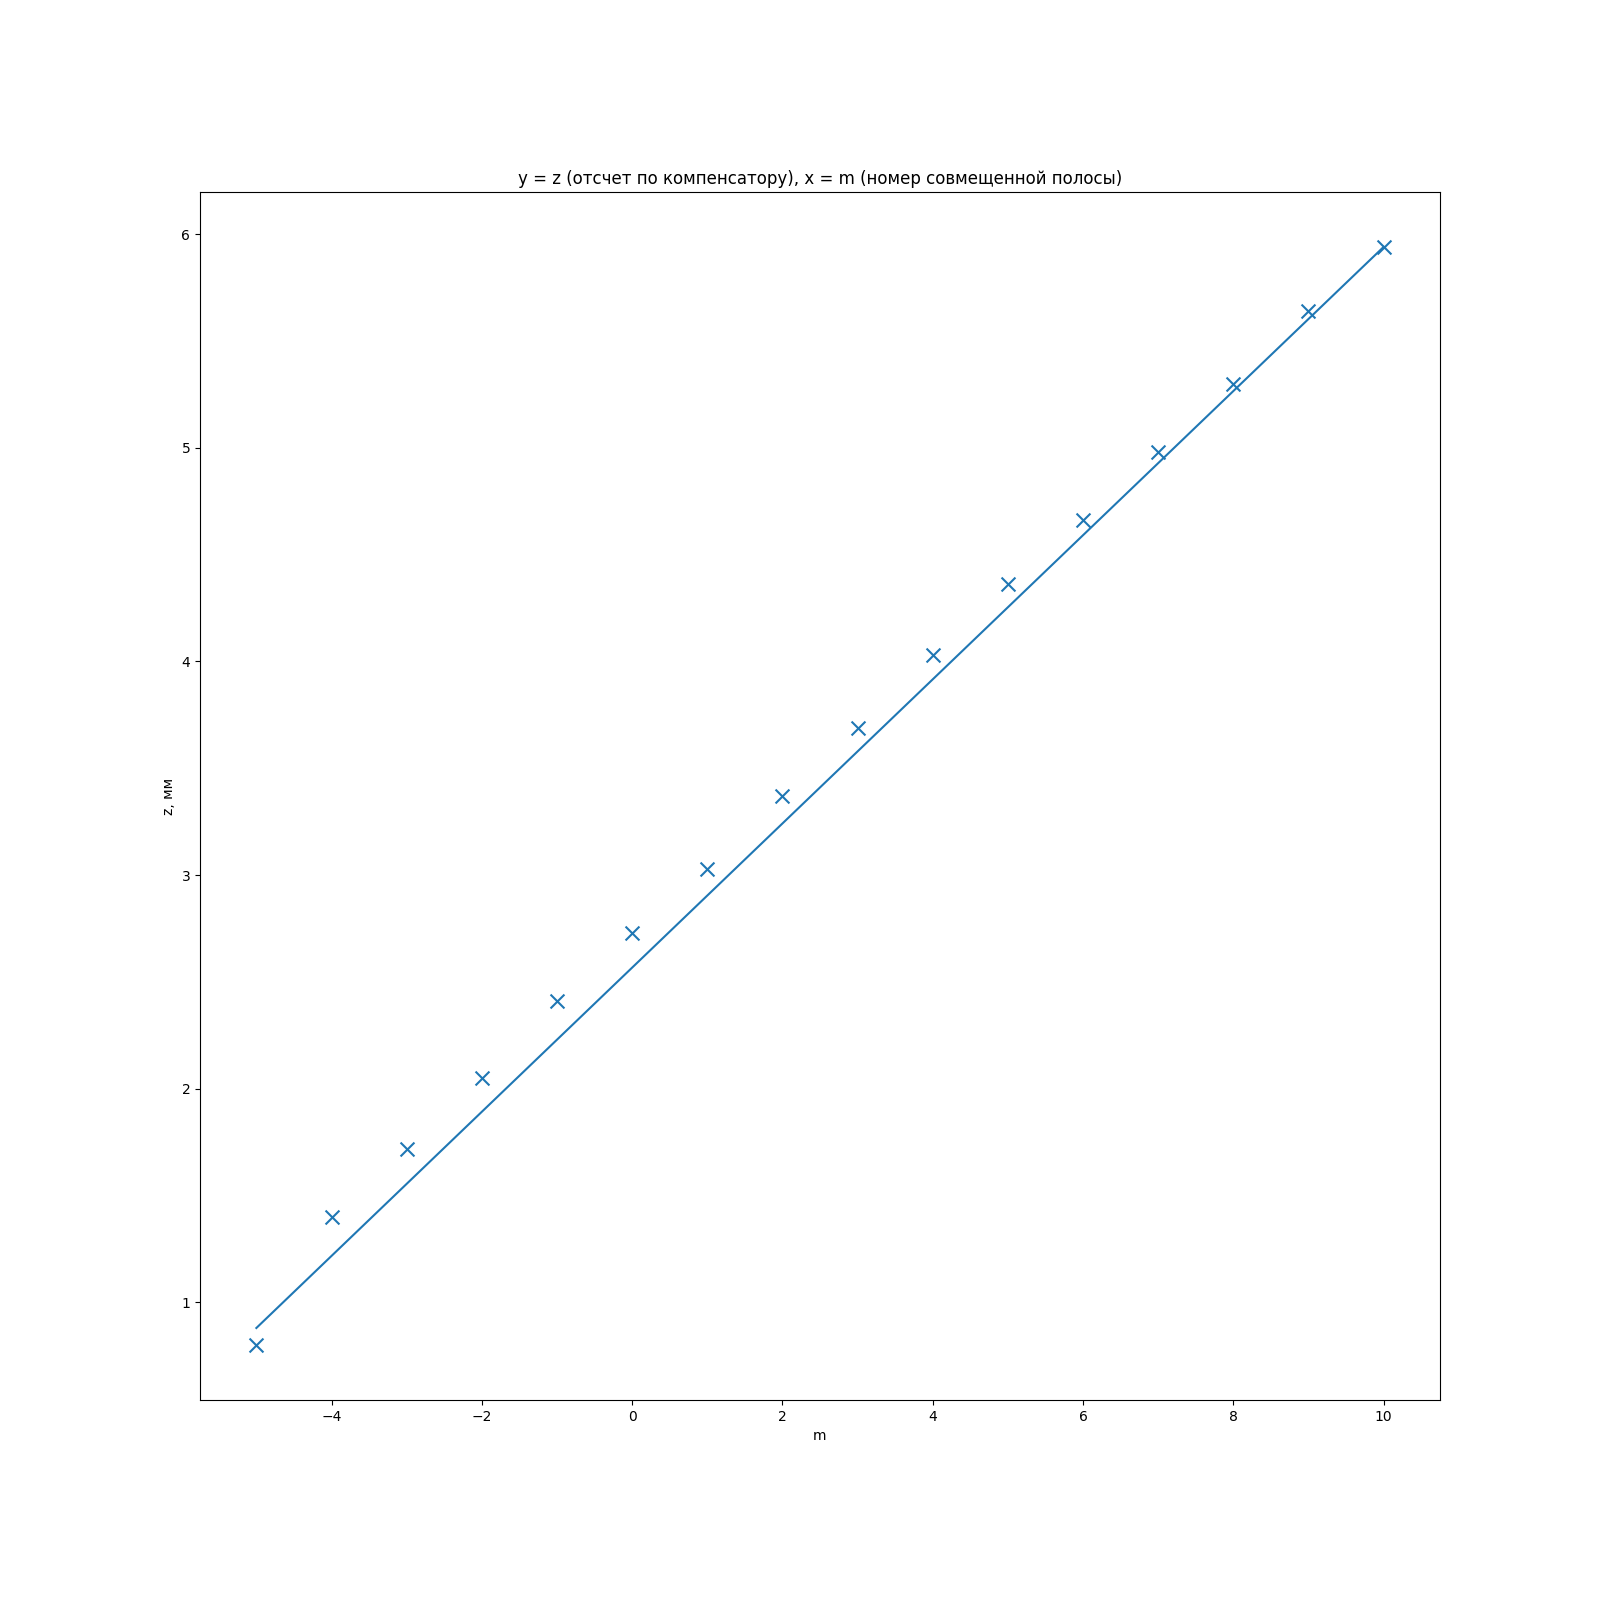
\includegraphics[scale = 0.45]{graph1.png}
        \centering
        \caption{Калибровочный график}
        \label{graph1}
    \end{figure}

    \item Построим график в координатах $x = \Delta P$ (от $+1000$ до $-1000$ мм в. ст.),$y = \Delta n$. Величину $\Delta n$ рассчитаем по формуле $\Delta n = \dfrac{\Delta}{l} = m \dfrac{\lambda}{l}$ с помощью калибровочного графика.
    
    \begin{figure}[!h]
        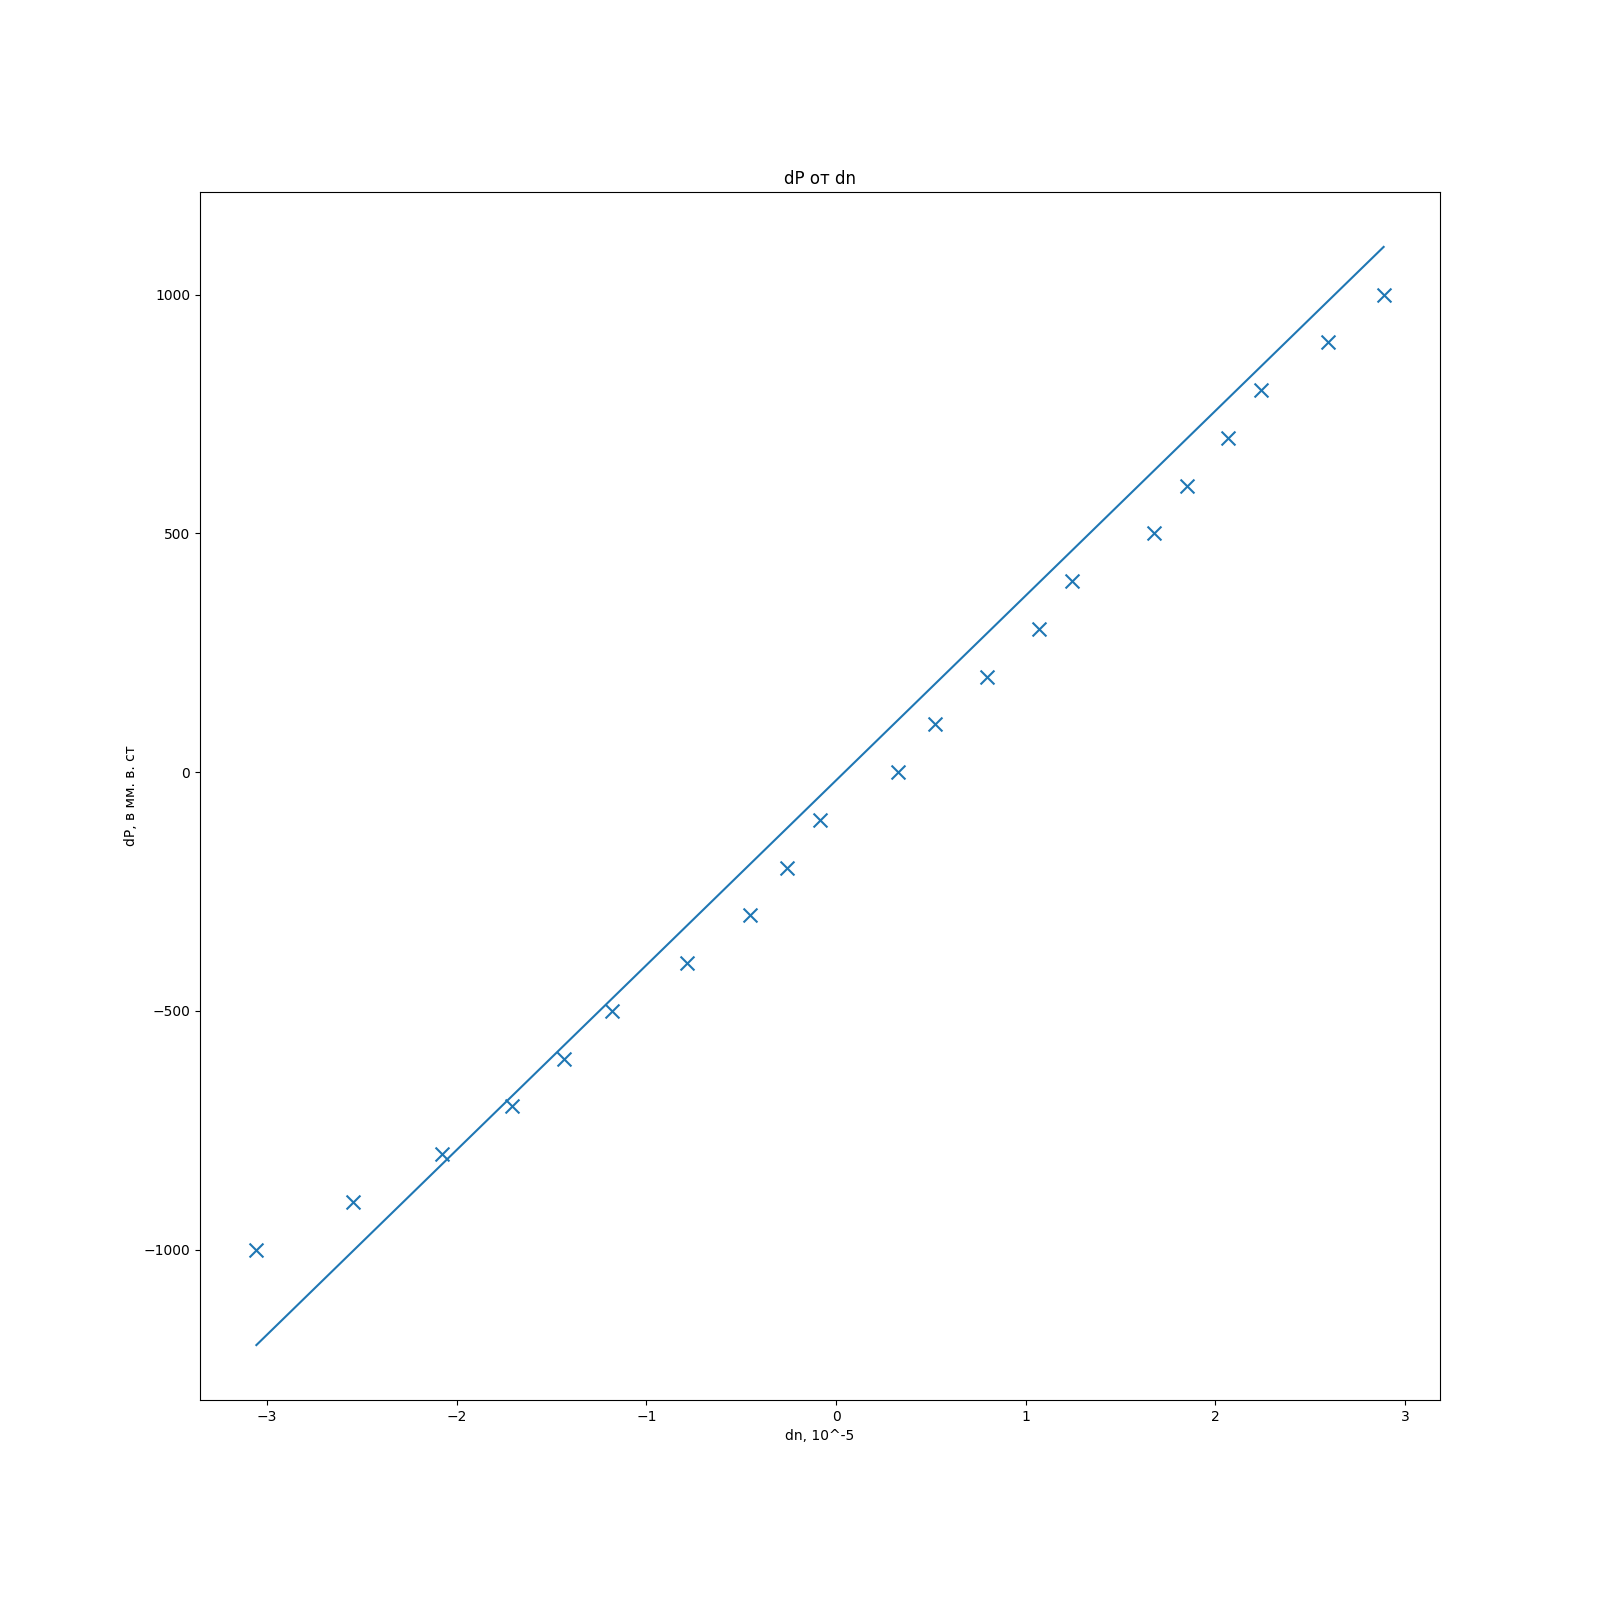
\includegraphics[scale = 0.45]{graph2.png}
        \centering
        \caption{$\Delta P$ от $\Delta n$}
        \label{graph2}
    \end{figure}

    По углу наклона рассчитаем среднюю поляризуемость молекулы воздуха, используя формулу $\Delta n = \dfrac{2 \pi \alpha}{kT}P$, а затем — показатель преломления воздуха в условиях опыта по формуле $n - 1 = 2 \pi \alpha \dfrac{P}{kT}$.

    $\alpha = (1.68 \pm 0.22) \cdot 10^{-30} \text{м}^3$

    $n = 1.00026 \pm 0.00004$

    Пересчитаем показатель преломления по формуле 
    \begin{equation*}
        \dfrac{n_0 - 1}{n - 1} = \dfrac{T}{T_0} \dfrac{P_0}{P}
    \end{equation*}
    к нормальным условиям:

    $n^0 = 1.00033 \pm 0.00004$

    \item Рассчитаем показатель преломления для углекислого газа в условиях опыта по формуле
    
    \begin{equation*}
        n = n_{возд} + \dfrac{\Delta}{l}
    \end{equation*}

    взяв показатель преломления воздуха, рассчитанный по результатам эксперимента.

    $n_{CO_2} = 1.00040 \pm 0.00004$

    Пересчитаем $n_{CO_2}$ к нормальным условиям:

    $n_{CO_2}^0 = 1.00051 \pm 0.00005$
    
    \item Оценим интервал $\Delta n$, доступный для измерений, исходя из возможностей компенсатора: минимальная величина $\Delta n$, доступная для измерений, определяется точностью компенсатора, максимальная — диапазоном его работы.
    
    Интервал, доступный для измерений: от $1.00037$ до $1.03$ 
\end{enumerate}
\end{document}